\section{Selection of viable regions}

After application of the correction method, each trace and its scalogram was submitted a manual control. During this control it was noticed that some traces still contained discontinuities which hampers correct data analysis for those traces. A table, which can be seen in \ref{ch:AppB}, was used to evaluate each region in each subject within both conditions, concerning the appearance of discontinuities in the trace after applied correction method and usability regarding further data processing.

With the aid of the evaluation table, five RIOs were chosen as valid for further data analysis. The criteria for this selection were, that those ROIs showed good response to the correction method and no discontinuity artifacts were visible shown in the scalogram. An example of this selection is illustrated on \figref{fig:selection}. The five selected ROIs are 10, 14, 20, 21 and 22, which are located in the back of the hand and can be seen in \figref{fig:roiHand}.

\begin{figure}[H]
	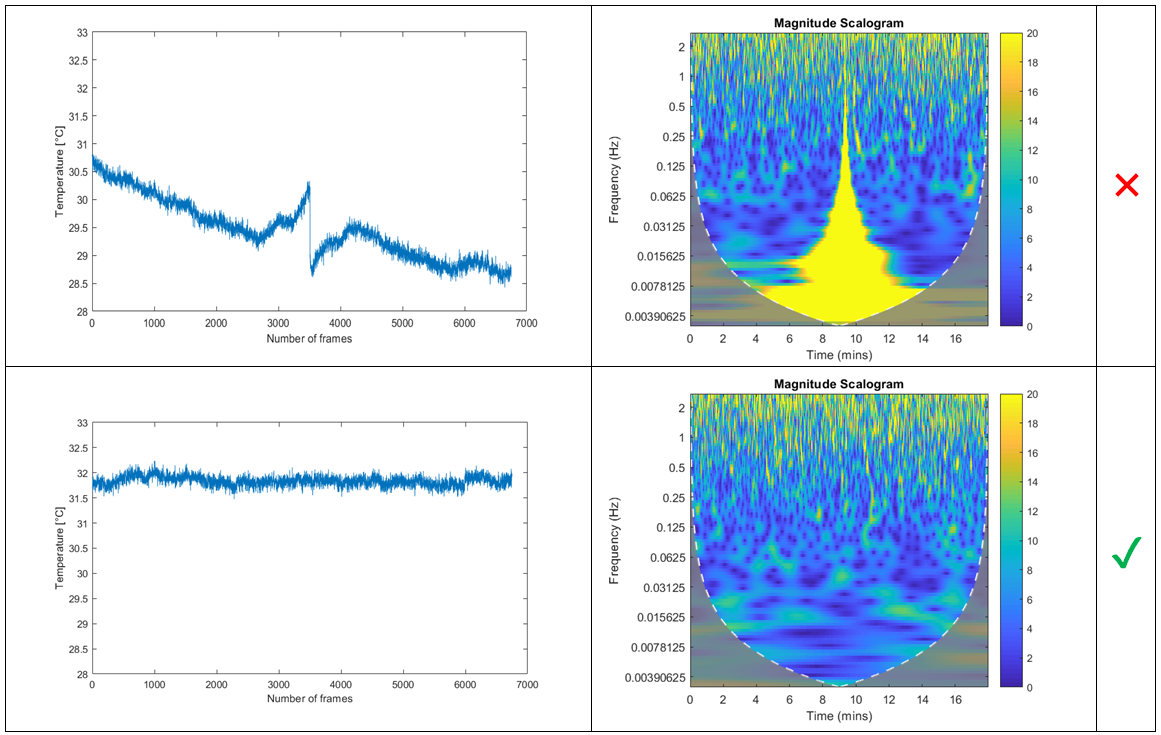
\includegraphics[width=0.7\textwidth]{figures/ROI_selection}
	\caption{Corrected traces from ROI 10 and 23, temperature plot with corresponding scalograms. ROI 23 was excluded and 10 accepted.}
	\label{fig:selection}
\end{figure} 